\section{Overview}

In Chapter \ref{chapter:supervised} I concluded that the number of examples has
a direct impact in the performance of a supervised \vsd~algorithm. I also
explained that small supervised corpora have a direct impact in both the
coverage and the tendency to overfit of a supervised model. To attack the
latter I saw in Chapter \ref{chapter:embeddings} that the use of word
embeddings, although decreasing performance in the test portion of the
supervised corpus, did help in the tendency to overfit of a model. In the
self-learning approach, word embeddings show an interesting performance as
well: even if coarse accuracy figures are more or less comparable for
hand-crafted features and for word embeddings, the latter have better recall in
minority classes and incorporate more informative features.

In Chapter \ref{chapter:self-learning} I explored self-learning as a joint
semi-supervised method. The original idea of using this method was to overcome
the problem regarding the model's coverage by adding new data, that is
automatically annotated, to the training set. The chapter also gave me more
insight of the benefits of using word embeddings as a representation when faced
with a task where the domain changes. However, there is a challenge in the
method of self-learning: the tendency of the method to add only examples of the
most frequent class.

This chapter introduces another semi-supervised joint learning framework: {\em
active learning}. Like self-learning, active learning consists in expanding the
training examples with new data provided by an unannotated corpus. Also, as a
wrapper method, it does so by training a model from labeled data and improving
that model with new labeled data obtained from the unlabeled corpus. 

The difference between self-learning and active learning lies in how the last
method labels the unlabeled data. This is not done automatically, but by the
means of an oracle, i.e. an annotator who has high certainty over the data it
is labeling (generally speaking, this is done by a human annotator, more
specifically a domain expert).

But this is not the only difference, since the way unlabeled instances are
selected for annotation also differs from the method used by self-learning.
While self-learning relies on the certainty the algorithm has over the data to
safely assume the given label is right, active learning seeks for data which,
once labeled, will yield the biggest improvement on the model. This data is
near the decision boundaries of the model and is generally more difficult to
tell it apart from data with other labels. 

One of the most popular techniques to select data that will improve the model
is {\em uncertainty sampling}. I briefly introduced it in
Chapter~\ref{chapter:general_background}. In this technique the underlying
hypothesis is that those instances on which the classifier has the least
confidence are the ones closest to the decision boundary and thus the ones to
make the most difference after being labeled.

In our setting, those instances which have the most impact on a model are
typically the ones that are underrepresented in the labeled dataset. And this
is precisely where active learning overcomes one of the problems of
self-learning: the bias to the most frequent class. As self-learning is a model
based on certainty, this implies that it will add mostly instances of the most
frequent class (typically the one the model has better certainty about, even if
only by probability). Active learning, on the other hand, helps the model spot
useful instances of those underrepresented classes in the labeled dataset and
provides the means to add them for a broader coverage.

Moreover, active learning not only adds examples of the pre-existing classes of
the model but of new classes as well. Remember in previous chapters I explained
that some classes of the SenSem corpus were filtered out because they did not
had enough occurrences in the supervised dataset. Besides those cases there are
also senses in the SenSem lexicon that did not have any examples in the
annotated corpus. As the labeled corpus is domain specific, this results in
the corpus not having examples of some of the possible senses. However, when
applying active learning over an unlabeled corpus of a general domain, examples
of these senses pop up in the flow of the algorithm. This is a common
phenomenon as the certainty the model has over those examples it never saw
before will be low, thus it will be picked up by the uncertainty sampling
technique. There are even senses that are directly not taken into account by
the resource, but these are left out as it is outside the scope of this thesis
because it requires the extension of the SenSem lexicon.

Regarding what is stated in the previous paragraph there is a remark to do
about self-learning. Recall that the last chapter showed that with the
self-learning model the certainty over new examples decreased in each
iteration. Thus it is possible that the self-learning algorithm was marking
those examples the model had less certainty about as part of the most frequent
class. However these examples were not even part of the initial labeled dataset
as the classes of those examples are not present.

This chapter will test the following hypothesis:

\begin{hypothesis}\label{hyp:active}
  Active learning improves the performance of a supervised model by reducing
  the bias of the initial dataset that is correlated to overfitting of the
  supervised model.
\end{hypothesis}

In order to accept or reject such hypothesis, I divide it in more specific
ones:

\begin{subhypothesis}\label{hyp:active:1}
  The representativity of the population for each class in the dataset is
  maintained through all the iterations of the algorithm.
\end{subhypothesis}

\begin{subhypothesis}\label{hyp:active:2}
  The active learning algorithm increases the number of features associated to
  the model more quickly than self-learning, which is an indicator of a quicker
  increment in the coverage of the model.
\end{subhypothesis}

These hypotheses will be tested using the following layout:

\begin{itemize}
  \item Experiment \ref{exp:active:2} records the number of occurrences per
    each class in the training dataset on every iteration of the active
    learning algorithm. The population of the classes is measured by the
    proportional count with respect to the whole training dataset. The results
    of this experiment, shown in Section \ref{sec:active:hyp:1}, serve to
    accept Hypothesis \ref{hyp:active:1} which states that the population of
    all the classes is maintained along the algorithm's iterations.
  \item Experiment \ref{exp:active:3} records the number of times a feature and
    a class occur together in an instance of the training dataset. I measure
    these results using two different metrics. First, in comparison to the
    results gathered from Experiment \ref{exp:self-learning:4} (which records
    the same data but for the self-learning algorithm), I use the normalized
    count of features by number of examples per iteration (Metric \ref{met:6}).
    It is necessary to normalize because the number of examples added in each
    active learning is much smaller than in self-learning, thus normalization
    is necessary for a meaningful comparison. On the other hand I analyze the
    PMI along the iterations for the classes and the features associated to it
    (Metric \ref{met:4}). The results are shown on Section
    \ref{sec:active:hyp:2} and serve to accept Hypothesis \ref{hyp:active:2}
    which states that the active learning algorithm improves the model's
    coverage quicker than self-learning.
\end{itemize}

In Section \ref{sec:active:previous} I revise some previous work in active
learning in general and also specifically applied to \vsd.

In Section \ref{sec:active:methodology} I go through the relevant items that
concern the experimentation in the chapter. Most of the methodology is very
similar to that in previous chapters, I mostly provide pointers to the sections
where this methodology is first described. In particular Section
\ref{sec:active:algorithm} explains the fine detail of the active learning
algorithm, e.g. the stopping criterion the algorithm uses, how the instances to
annotate are selected and how the annotation is carried out, as well as some of
the difficulties of the annotation. 

Section \ref{sec:active:results} reports the results of the experiments and
analyzes them in order to accept the stated hypotheses of the chapter.

Finally Section \ref{sec:active:conclusions} draws the conclusions of this
chapter, recapitulating the Hypotheses and the implications of accepting or
rejecting them according to the evidence gathered in the results. It states the
shortcomings of the methods explored in this chapter and what I want to
accomplish on the next. It ends by outlining future work.

\section{Relevant work}\label{sec:active:previous}

Active learning is a task for semi-supervised learning, based on the key idea
that if the learning algorithm is allowed to choose the data from which it
learns it will perform better with less training. A very complete survey in the
area is the one done by Settles \cite{settles.tr09}. It covers all the main
topics in the area of active learning.

A particularly important subject in active learning is the strategy to select
the instances to present to the oracle. Different strategies have been studied,
being {\em uncertainty sampling} the most intuitive and popular one
\cite{Lewis94heterogeneousuncertainty} and the one used in this chapter. For
other strategies refer to Section \ref{sec:general_background:active} of
Chapter \ref{chapter:general_background}.

One of the main problems in applying active learning to natural language
processing tasks is class imbalance, something common in the are. In this
cases, uncertainty sampling not always proves being the best way to select data
given some difficulties it arises as I will explain in Section
\ref{sec:active:difficulties}. There are some approaches to deal with it, but
nothing definitive.

In particular, Dligach and Palmer \cite{dligach2011good} applied active
learning to verb sense disambiguation. They explored the benefits of using an
unsupervised language model to select seed examples as a starting corpus for an
iterative active learning approach.

\section{Methodology}\label{sec:active:methodology}

This chapter explores the use of active learning with a human annotator to
expand a model trained with labeled data. Like the self-learning algorithm in
the previous chapter, active learning is also a {\em wrapper}. The algorithm
uses a supervised classifier to select instances from the unlabeled data and
gives it to a human to verify it.

The objective of this chapter is to show the tendencies I have found using
active learning. I do not present an exhaustive analysis of active learning, as
it requires annotating resources using human experts which I are outside the
possibilities of research of this thesis. The idea is to analyze preliminary
results which can help as an initial start for future work using more
resources.

\subsection{Resources}\label{sec:active:resources}

In this chapter I keep using the datasets I have been working on so far: the
SenSem corpus as labeled corpus and SBWCE as the unlabeled.

Analyzing active learning was the main reason to reduce the analysis to some of
the lemmas in the lexicon. The selected lemmas on which I make my analysis are:
``explicar'', ``pensar'', ````acceder'''', ``llegar'', ``buscar'' and
``facilitar''. A detailed explanation of this is done in Section
\ref{sec:self-learning:resources}, please refer to it for more information.

The SenSem corpus is used as the annotated seed on which the active learning
algorithm starts. For a detailed description of the resource please refer to
Section \ref{sec:supervised:sensem}.

The unlabeled data source for new instances to give to the human expert to
manually annotate is taken from the SBWCE corpus. Please refer to Section
\ref{sec:embeddings:sbwce} for more details on the corpus. The corpus is the
one pre-processed with Freeling obtained by the methodology described in
Section \ref{sec:self-learning:sbwce}. Please refer to that section for more
details on how this is done.

\subsection{Features}

The features used in this part are the same ones used in the previous chapters.
Both hand-crafted features using the hashing trick and word embeddings follow
what has been discussed in all the previous chapters.

For more information on the detail of what are the hand-crafted features used
in this chapter please refer to Section \ref{sec:supervised:features}. For
detailed information on how to deal with the expansion of features given by the
new examples added to the model please refer to Section
\ref{sec:self-learning:handcrafted}.

The word embeddings are the ones trained from the journalistic corpus described
in detail in Section \ref{sec:embeddings:journal}. The method for combining
them into an instance is the concatenation of word vectors described in Section
\ref{sec:embeddings:embeddings}.

\subsection{Classifiers}

As in self-learning, active learning is a wrapper method that is built around a
supervised classifier. The selected classifier is the same as in the previous
chapters. I use a multilayer perceptron with three layers of size 500, 250 and
100 each.

\subsection{Active learning algorithm}\label{sec:active:algorithm}

The active learning algorithm follows the same structure as the self-learning
algorithm described in Section \ref{sec:self-learning:algorithm}, taking as
input almost the same initial parameters:

\begin{itemize}
  \item A labeled training dataset to train the initial supervised model.
  \item A labeled test dataset to report the model performance before and after
    finishing all the iterations of the self-learning algorithm.
  \item An unlabeled dataset to get the new data to annotate automatically.
  \item A probabilistic classification algorithm, to use in the process of
    automatic annotation.
  \item A maximum number of elements to annotate each iteration.
  \item A tolerance error for the stopping criterion.
\end{itemize}

The fundamental differences in this case reside in the following items: (i) how
the model selects instances to label from the unlabeled dataset, (ii) how those
instances are annotated, (iii) how the model decides whether new instances are
to be included in the training corpus, (iv) how the algorithm finishes.

\subsubsection{Instance selection and annotation}

In each iteration of the algorithm, once the classifier is trained with the
examples gathered so far (both part of the initial seed dataset or from the
oracle's annotations) the algorithm applies the classifier to the whole pool of
unannotated data. From the automatic annotation of that pool of unlabeled
examples, the algorithm takes the ones the classifier is less certain about and
presents them to the oracle for manual annotation. This is called {\em
uncertainty sampling}, i.e. selecting those instances for which the certainty
of the classifier is low. It is assumed that those instances are near the
decision boundaries of the model. The intuition behind using this method
instead of randomly giving the oracle examples to annotate is that these
examples will have the largest impact on the final model, that is, the model
will improve its accuracy the most. This is because the classifier gains
confidence on those classes and instances it has less information about in the
seed labeled corpus. This is a way to optimize learning with a given amount of
training data, by improving the quality (not the quantity) of the training
examples.

Unlike self-learning, which selects all the instances over a threshold, in
active learning there is a maximum number of possible instances. It is given as
an initial parameter of the algorithm. This number is selected empirically and
should be large enough to make a difference in the new model but not too big to
have the oracle devoting too much time annotating, since active learning gives
an intelligent way to minimize the annotation effort. After some
experimentation, the number of 10 examples per iteration was selected as the
base for the experiments in this chapter.

The oracle annotates the examples selected by the active learning algorithm,
which are then added to the model. There is however a problem, as I explained
before: the initial annotated corpus may not have a correct label for some
examples because it was not considered originally when designing the lexicon.
In those cases, to reduce the number of possibilities to consider and as it is
outside the scope of this thesis to extend the resource, I decided to ignore
examples belonging to an sense not present in SenSem.

\subsubsection{Validation of the model and early stopping}

Once the instances are annotated by the oracle, the next step is, like in
self-learning, to add them as new training examples. However, the algorithm
first checks the impact of adding these new examples to the model, by assessing
the performance of the model with the bigger training corpus.

For self-learning, this was done using a validation dataset extracted from the
original dataset. I originally thought about using cross validation over the
training dataset in self-learning, but finally I abandoned the idea. The
tendency of the self-learning algorithm to add everything as part of the most
frequent class may have introduced bias in that method of validation.

For active learning however this is not a problem. As the annotation is not
left to the classifier but to a human, the tendency to annotate everything as
the most frequent class does not prevail as much. I decided then to use
cross-validation over the training examples and see the mean of the
misclassification error obtained from it as the metric to validate the impact
of the new training examples in the model. 

The main reason to use cross validation over the training dataset and not a
validation dataset like in self-learning is because unlike in self-learning,
this algorithm may add examples of classes not seen by the model so far.
Remember some senses were filtered out from the SenSem corpus because they did
not have enough available instances. Moreover, some of the senses in the
lexicon do not have any examples at all. Well, these senses occur in a larger
corpus like SBWCE, and as the classifier will not have enough information
initially over those senses, it is likely that examples of those are chosen to
give to the oracle using the uncertainty sampling technique.

As new examples of unseen classes may be added to the training data this might
result on the validation corpus not reflecting the model's real performance.
The reason behind this is that the validation corpus does not have any
information regarding the new unseen classes the model is adding.

Once the algorithm calculates the misclassification error from the
cross-validation over the training dataset it applies the same principle the
self-learning algorithm did, it compares it to the minimum error obtained so
far and gives a tolerance of maximum 10\% less than random chance. If the error
in the new model is larger than that, the algorithm discards the model and
returns the last model obtained so far. As it requires human annotation, the
algorithm also provides the option for the human to stop iterations whenever he
wants.

\subsubsection{Difficulties in the annotation}\label{sec:active:difficulties}

There were two major difficulties when dealing with the annotation of the
examples selected by the algorithm based on high uncertainty: ambiguity and
coverage of the classes available in the resource.

Since the inventory of senses is human given, it is arbitrary, shaped by the
humans creating the resource and the final objective such resource has. This
means that depending on these variables, the inventory of senses may be coarse
or fine-grained. This of course affects the possibilities to annotate, as a
more coarse inventory may fall in the problem of having senses that are
suitable for more than one sense. As the algorithm selected those instances
that are near decision boundaries, a common problem is giving the oracle
examples that are ambiguous even for the oracle to discern.

Besides the problem of having senses with blurry decision boundaries, which
overlap with each other, the other problem the resource may have is lack of
coverage. Thus there are some examples that are not suitable for any of the
senses given in the resource. This is particularly common since an important
part of the SBWCE corpus consists on books written in old Spanish (i.e. the
ones compiled in the Wikisource initiative). Thus there are some senses which
fell into disuse and were not considered in the construction of the resource.

\subsection{Experiments}\label{sec:active:experiments}

There are three major experiments I did in this chapter: one to compare the
performance of the active learning algorithm with the self-learning algorithm,
and two others to test the hypotheses.

First, Experiment \ref{exp:active:1} is very similar to Experiment
\ref{exp:self-learning:1} in Chapter \ref{chapter:self-learning}. The
experiment is not aimed at testing any of the hypotheses of this chapter but
rather as a comparison with the previous chapter. It basically tests the active
learning algorithm and how it affects the performance of the supervised
classifier over the held-out test data.

\begin{experiment}\label{exp:active:1}
  \begin{enumexp}
    \item Train a model with the supervised training dataset.
    \item Evaluate the model over the test dataset.
    \item Run the active algorithm until it stops.
    \item Evaluate the model obtained with the active algorithm over the test
      dataset.
  \end{enumexp}
\end{experiment}

Experiment \ref{exp:active:2} is the first experiment to test a hypothesis in
this chapter. The experiment is to evaluate the representativity of the
population for each class across the active learning iterations. It is done to
test Hypothesis \ref{hyp:active:1}, which states that this representativity is
maintained through all the iterations of the algorithm. This experiment is
based on Experiment \ref{exp:self-learning:5} in the previous chapter.

\begin{experiment}\label{exp:active:2}
  \begin{enumexp}
    \item Record the number of times each class occurs in the supervised
      training dataset.
    \item Run an iteration of the active learning algorithm.
    \item Record the number of times each class occurs in the new training
      dataset comprised of the supervised data and the new annotated
      examples.
    \item Repeat the previous step for each iteration of the algorithm.
  \end{enumexp}
\end{experiment}

Finally, to test Hypothesis \ref{hyp:active:2} regarding the number and
association of features to classes, there is Experiment \ref{exp:active:3},
which is based on Experiment \ref{exp:self-learning:4} in the previous chapter.
The experiment records the number of times each tuple of classes and features
appear in the dataset.

\begin{experiment}\label{exp:active:3}
  \begin{enumexp}
    \item Record the number of times a tuple $(class, feature)$ occurs for each
      class and each feature of the supervised training dataset.
    \item Run an iteration of the active learning algorithm.
    \item Record the number of times a tuple $(class, feature)$ occurs for each
      class and each features of the training dataset comprised of the
      supervised data and the automatically annotated instances.
    \item Repeat the previous step for each iteration of the algorithm.
  \end{enumexp}
\end{experiment}

\subsection{Metrics}\label{sec:active:metrics}

To report the results of Experiment \ref{exp:active:1} I use the F1-score for
each class in the test dataset of the token lemmas, for each of the three
algorithms: supervised, self-learning and active learning.

For Hypothesis \ref{hyp:active:2}, which compares the features association that
comes from the active learning iterations, I mainly focus on two metrics. One
is Metric \ref{met:4}, which calculates the PMI between features and classes
and associates each feature to the class it has a higher PMI with. The other is
Metric \ref{met:6} which is the normalized count of features by examples: 

\begin{metric}\label{met:6}
  \begin{enummet}
    \item Count the total number of features in an iteration of a joint
      learning algorithm.
    \item Divide it by the total number of examples added in that same
      iteration.
  \end{enummet}
\end{metric}

\section{Analysis of results}\label{sec:active:results}

This section reports the results obtained by the experiment described before,
with the mentioned metrics. There is an important remark to do on these
results. This is an exploratory and preliminary work. Active learning, as it
requires resources of annotation from a domain expert, is very costly. For this
thesis, the amount of effort that could be devoted to annotation was very
limited, so active learning is presented here as a proof of concept, showing
tendencies instead of clearly defined results. Results however are interesting
to show and analyze. Once again, the visualization and metrics used here can
obscure some aspects of the results in favor or others. I will try to give the
most impartial analysis over this data.

\subsection{Performance comparison for self-learning and active learning}

Before delving into the analysis of the hypotheses of this chapter, I want to
do a quick review on how the two different algorithms seen so far
(self-learning and active learning) compare in terms of performance against the
supervised algorithm. This is done to establish some common ground for all the
joint learning algorithms.

These results are gathered from Experiment \ref{exp:active:1}, which measures
the performance of the model by using F1-score per class, showing the
performance for the most frequent, second most frequent and third most frequent
class of the lemma. I do this because these are the classes of the token lemmas
that were not filtered out in the preprocessing of the corpus. From the 6 token
lemmas, 4 of them have only two senses with instances in the labeled dataset
(``acceder'', ``buscar'', ``explicar'', and ``facilitar''), and only 2 of them
have 3 senses with instances in the dataset (``llegar'' and ``pensar'').

\begin{figure}[htb!]
  \centering
  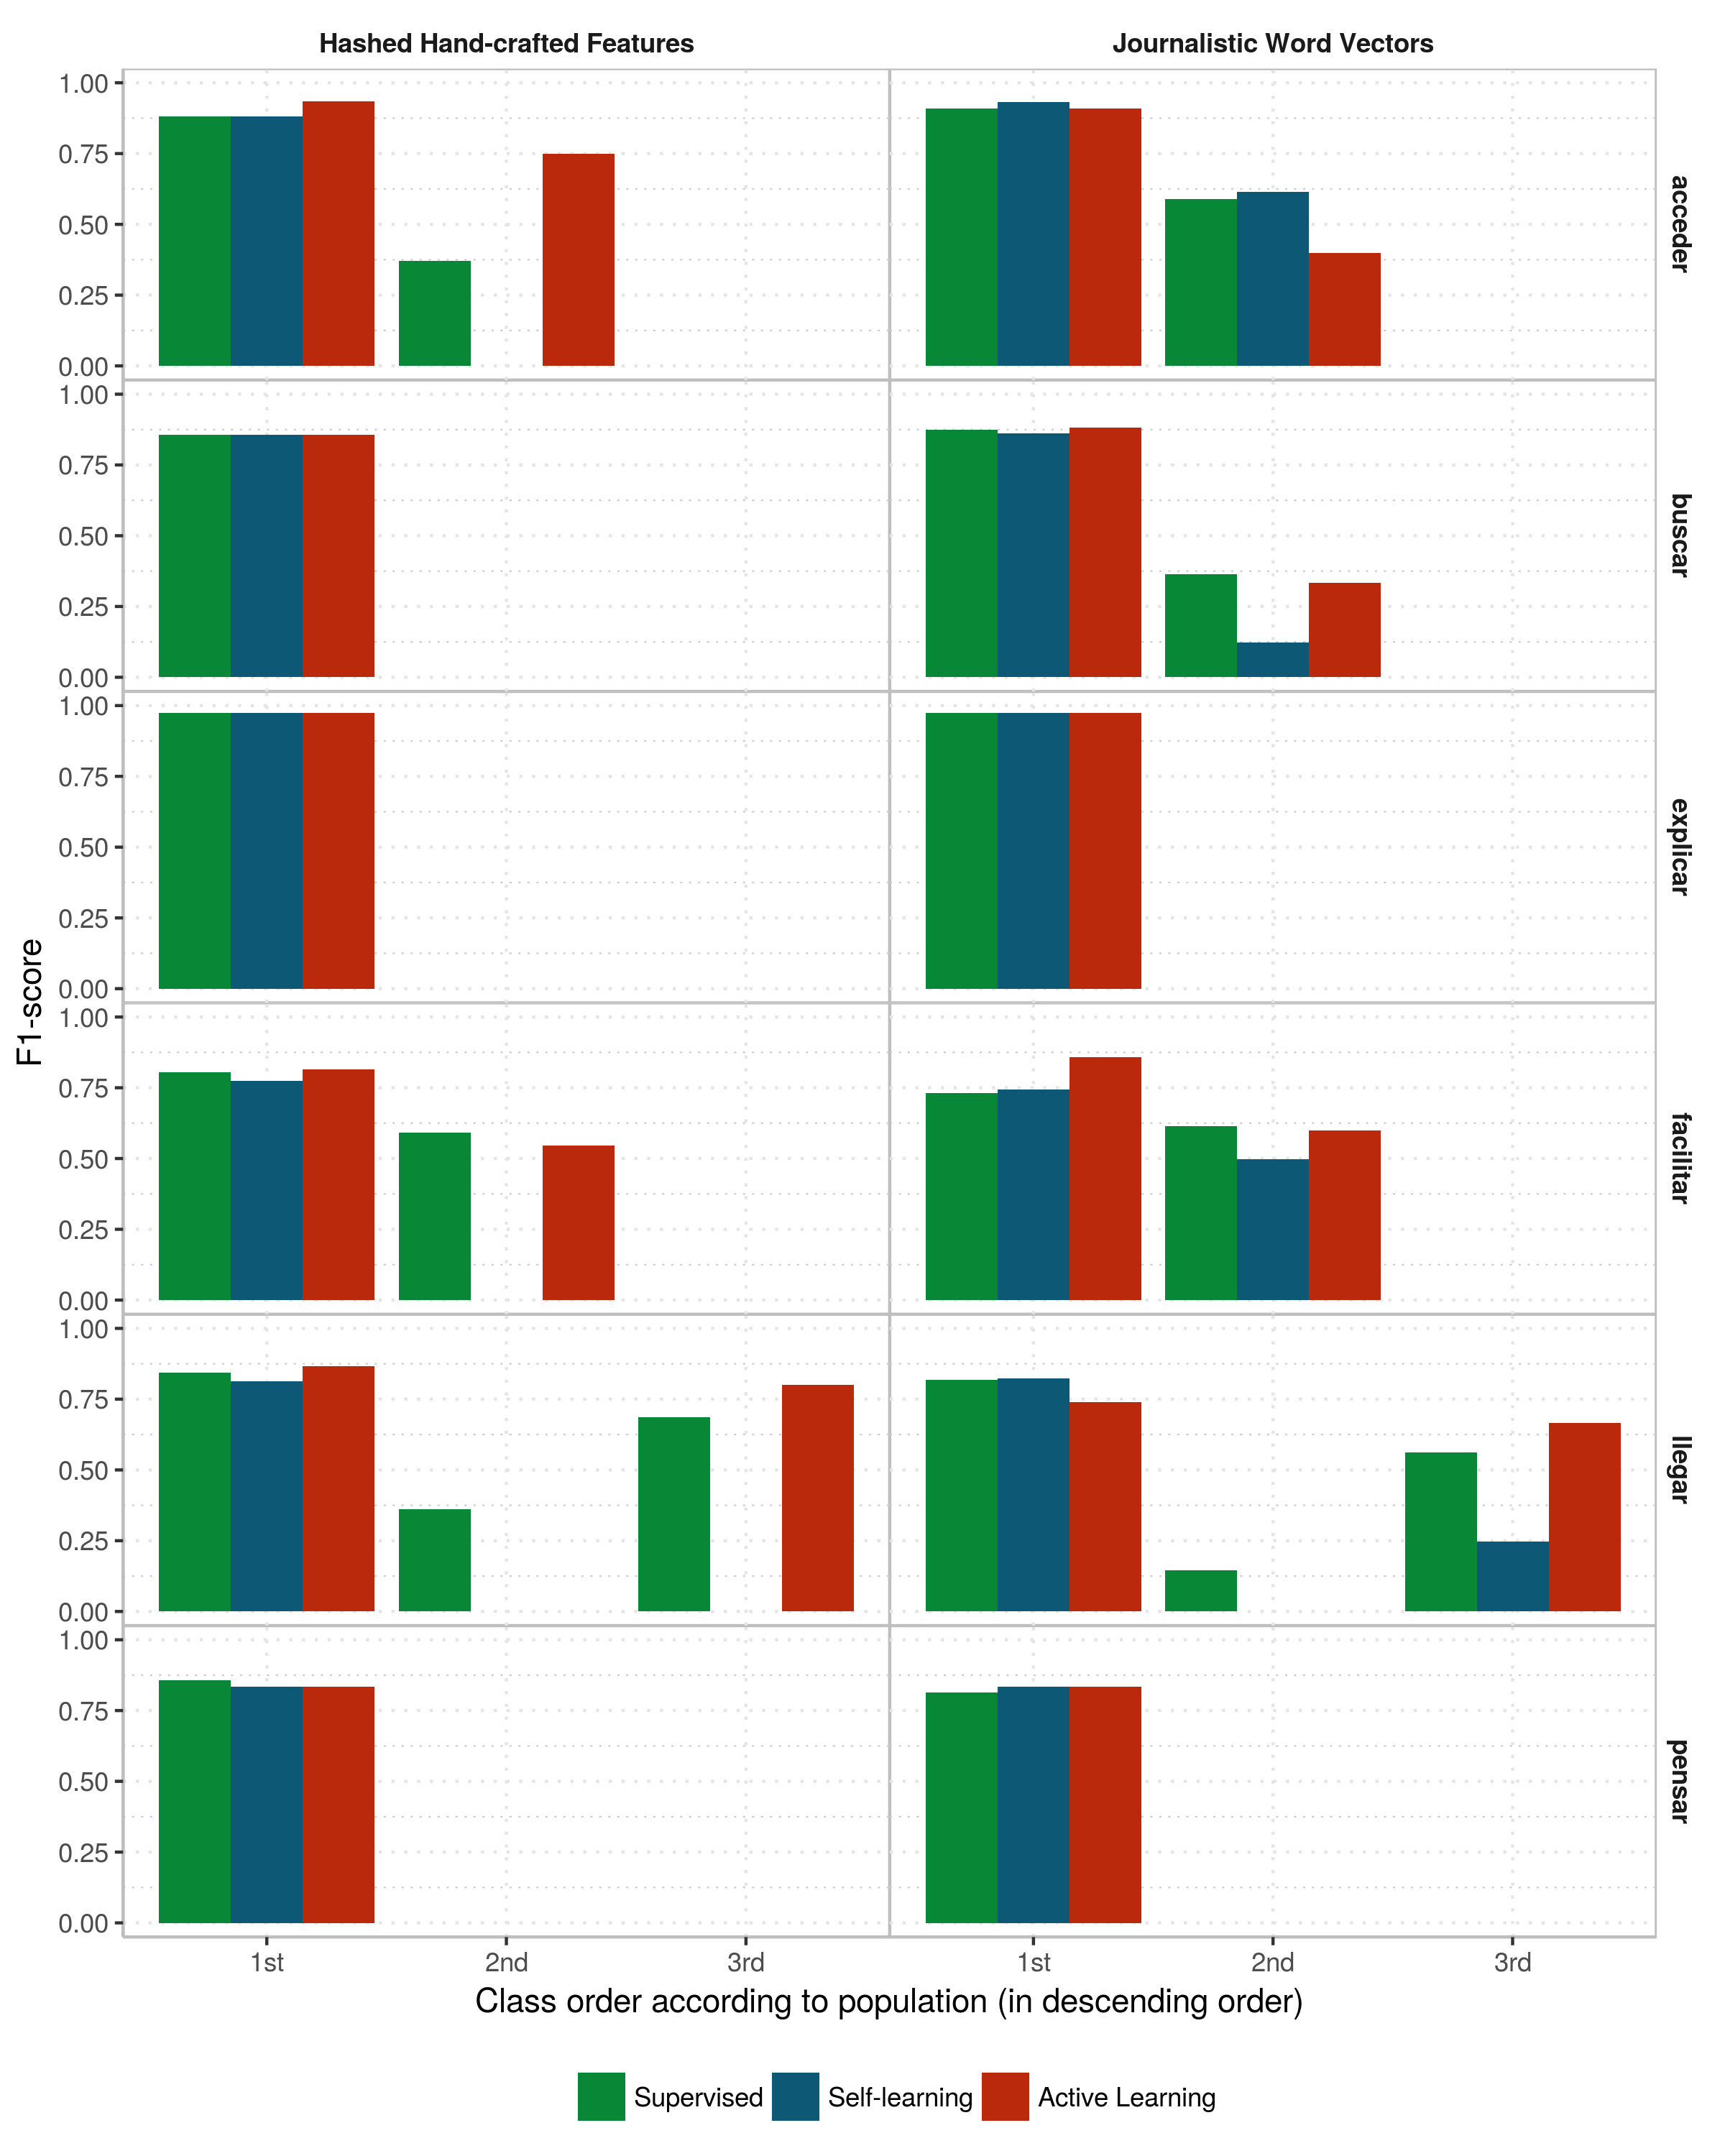
\includegraphics[height=0.9\textheight,width=\textwidth,keepaspectratio]
    {plots/active/per_sense_fscore}
  \caption{Comparison of macro and weighted average F1-score for supervised,
  self-learning and active learning}
  \label{fig:active:performance}
\end{figure}

Figure \ref{fig:active:performance} shows the F1-score macro and weighted
average for supervised, self-learning and active learning over the test
dataset. In this case, ``supervised'' is the evaluation of the model in the
initial iteration of any of the joint learning algorithms (as it is the same
for both, i.e. only using the manually labeled data). The self-learning/active
learning bars represent the performance of the model over the held-out test
dataset after finishing the iterations of the corresponding algorithm. The
structure of the graphic is as follows:

\begin{itemize}
  \item Each row shows the results for a token lemma: ``acceder'', ``buscar'',
    ``explicar'', ``facilitar'', ``llegar'', and ``pensar''.
  \item Each column stands for a feature representation: hand-crafted hashed
    features and journalistic word vectors.
  \item Each group of bars in each plot represents the class (i.e. sense) for
    that lemma. These are ordered according to number of occurrences of the
    class in the dataset.
  \item Each bar plot in a different color inside a group represents the
    algorithm: supervised (i.e. evaluation moment of the initial iteration),
    self-learning (i.e. evaluation moment of the final iteration after
    self-learning finishes), and active learning (i.e. evaluation moment of the
    final iteration after active learning finishes).
  \item The height of the bar represents the value of the F1-score per each
    class.
\end{itemize}

Recall again that only the last two rows of the graphic represent lemmas with 3
senses (i.e. ``llegar'' and ``pensar''). The first four lemmas can at most show
results for two senses.

In general, active learning performs better than self-learning and even better
than supervised in some cases for both the most frequent class and the less
frequent classes. It might be that active learning performed better than
supervised learning simply because the amount of annotated examples increases.
However, the amount of annotated examples also increases for self-learning, but
it does not impact in the performance. This is a clear sign that the selection
of examples to give to the oracle to annotate is in the right track, because it
does have a visible impact in the performance of the resulting model, beyond
the mere increment in the number of annotated examples.

Once again, like in the previous chapter, word embeddings still show better
overall performance than hand-crafted features: minority senses are better
represented, without an important loss of performance in majority senses. In
combination with active learning, word embeddings become particularly useful,
as they properly characterize minority senses. 

Now that I have a base comparison of the two algorithms I have strong evidence
that active learning is better for the performance of the model. To check why
this is the case I will look further into the hypotheses.

\subsection{Hypothesis \ref{hyp:active:1}}\label{sec:active:hyp:1}

This section tests Hypothesis \ref{hyp:active:1}. The hypothesis states that
the representativity of each class's population in the training dataset is
maintained through all the algorithm iterations. Recall that for the
self-learning algorithm I found evidence to accept Hypothesis
\ref{hyp:self-learning:6}, which states the opposite of Hypothesis
\ref{hyp:active:1}. 

More precisely, I established that the fact that self-learning was not
representing all classes properly was the cause for the self-learning degrading
the performance of the less frequent classes, as stated in Hypothesis
\ref{hyp:self-learning:5} in the previous chapter. As I saw in the previous
section, this is not the case for active learning, since it does improve on the
performance of classes other than the most frequent one.

I show the results for Hypothesis \ref{hyp:active:1} to assess whether the
reason behind the improvement in performance is effectively a better
representation of the minority classes with the active learning algorithm.

To test the hypothesis I measure the results obtained after doing Experiment
\ref{exp:active:2} which records the number of instances each of the classes
has in the training dataset after each active learning iteration.

Once again, as in the previous chapter, to visualize these results I use two
techniques to show what, for me, is relevant on the checking of the Hypothesis:
the proportional count of the number of instances per class along the
iterations, and the proportional number of instances added for each class per
iteration. These two results will allow to accept Hypothesis
\ref{hyp:active:1}.

\subsubsection{Classes' population distribution across iterations}

\begin{figure}[htb!]
  \centering
  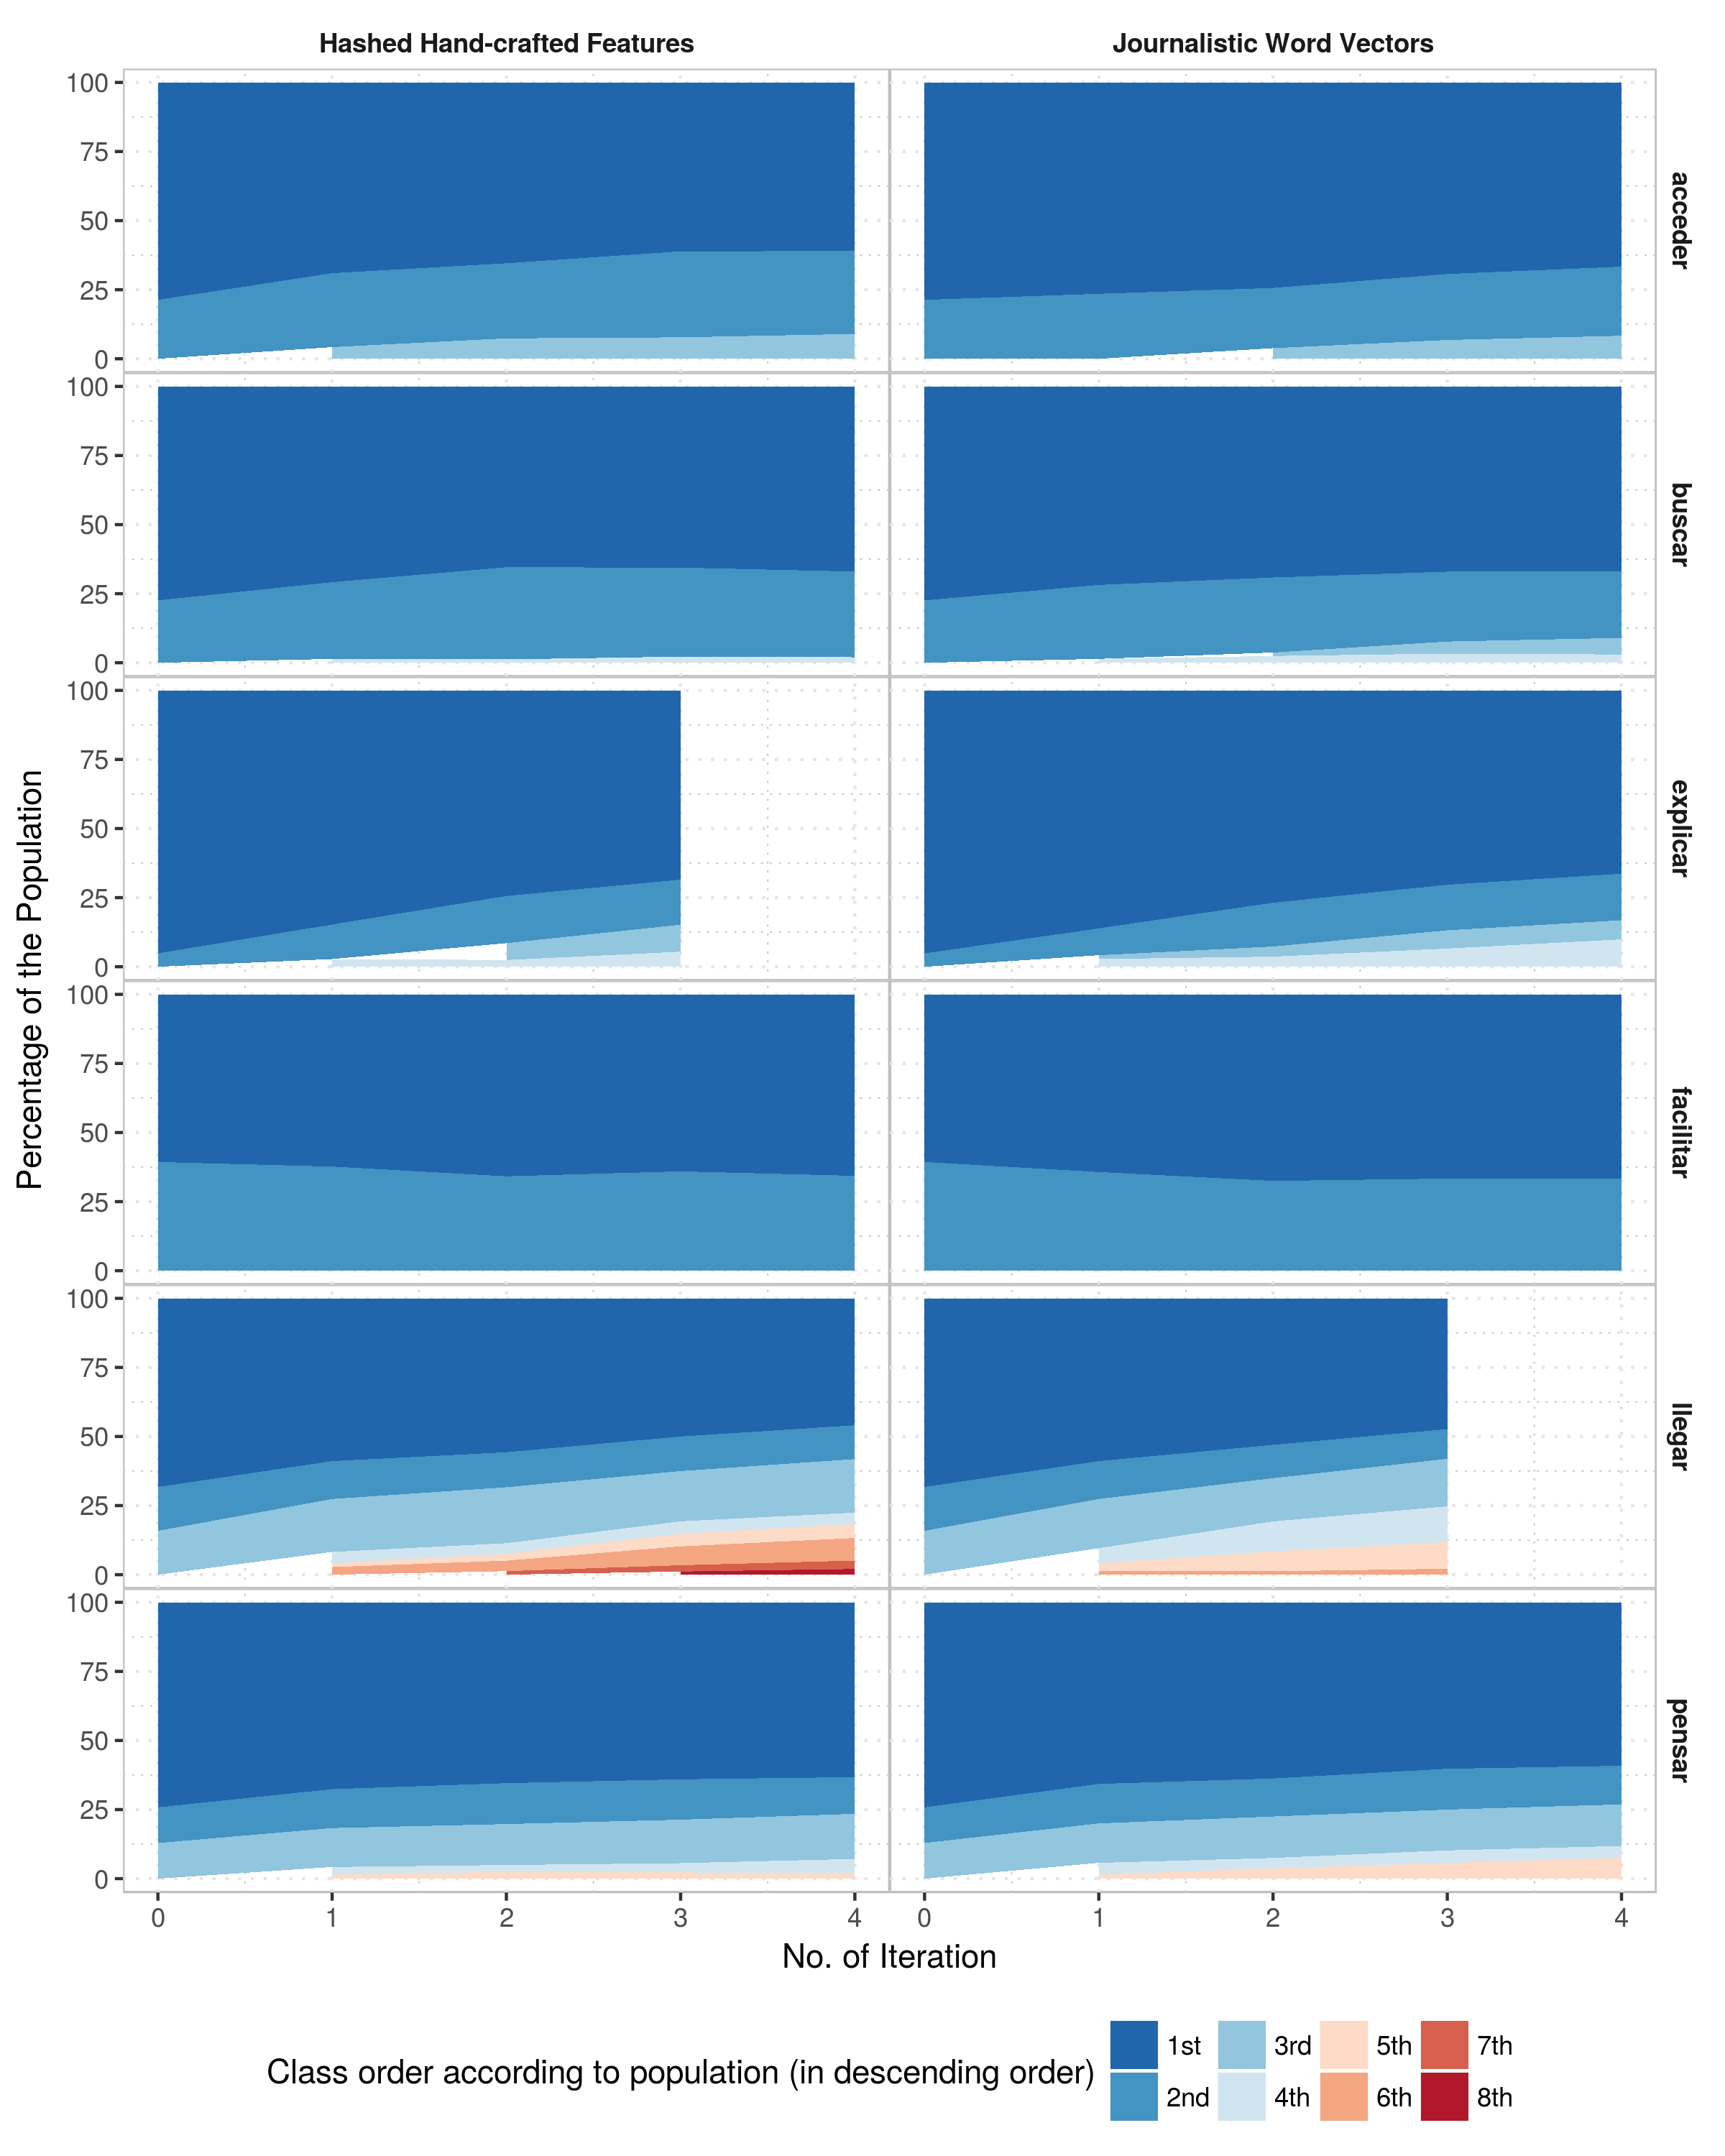
\includegraphics[height=0.9\textheight,width=\textwidth,keepaspectratio]
    {plots/active/population_distribution}
  \caption{Distribution of the classes' population across active learning
  algorithm's iteration as a proportion of the whole training dataset}
  \label{fig:active:population_distribution}
\end{figure}

Figure \ref{fig:active:population_distribution} shows the distribution of the
population of the classes across the active learning iterations. Each class's
population is represented as the proportion of the total number of examples in
the training dataset for that iteration. The plot is a stacked area plot that
follows this structure:

\begin{itemize}
  \item Each row shows the results for a token lemma: ``acceder'', ``buscar'',
    ``explicar'', ``facilitar'', ``llegar'', and ``pensar''.
  \item Each column stands for a feature representation: hand-crafted hashed
    features and journalistic word vectors.
  \item The x-coordinate represents the iteration in the self-learning
    algorithm.
  \item The y-coordinate represents the percentage of population.
  \item Each area of a different color represents the proportion of examples
    for each of the classes in the dataset. The classes again are ordered
    according to number of examples in the original supervised dataset.
\end{itemize}

The first thing to notice from the figure, specially compared to the similar
figure of the previous chapter, is the number of iterations. While for
self-learning iterations could go up to 100, for active learning I only did the
annotations for 4 iterations total (plus the initial iteration, which is
represented in the number 0). This is why I say that the work done for active
learning is mostly exploratory.

Note that there are two cases where the iterations are less: ``explicar'' (for
the hand-crafted features representation) and ``llegar'' (for the word
embeddings representation). In this cases the iteration finished before because
the stopping criterion of the validation error was met.

The second noticeable thing in the figure is the increase in the number of
classes that occur as the iterations advance. This is a result of what I
explained before: the algorithm selects those instances on which it does not
have enough information, which are generally those that are not part of the
original supervised corpus. This is a marked difference with self-learning: in
active learning the less frequent classes also grow in number of examples
through the iterations, not only the most frequent one.

\subsubsection{Population added per sense per iteration}

\begin{figure}[htb!]
  \centering
  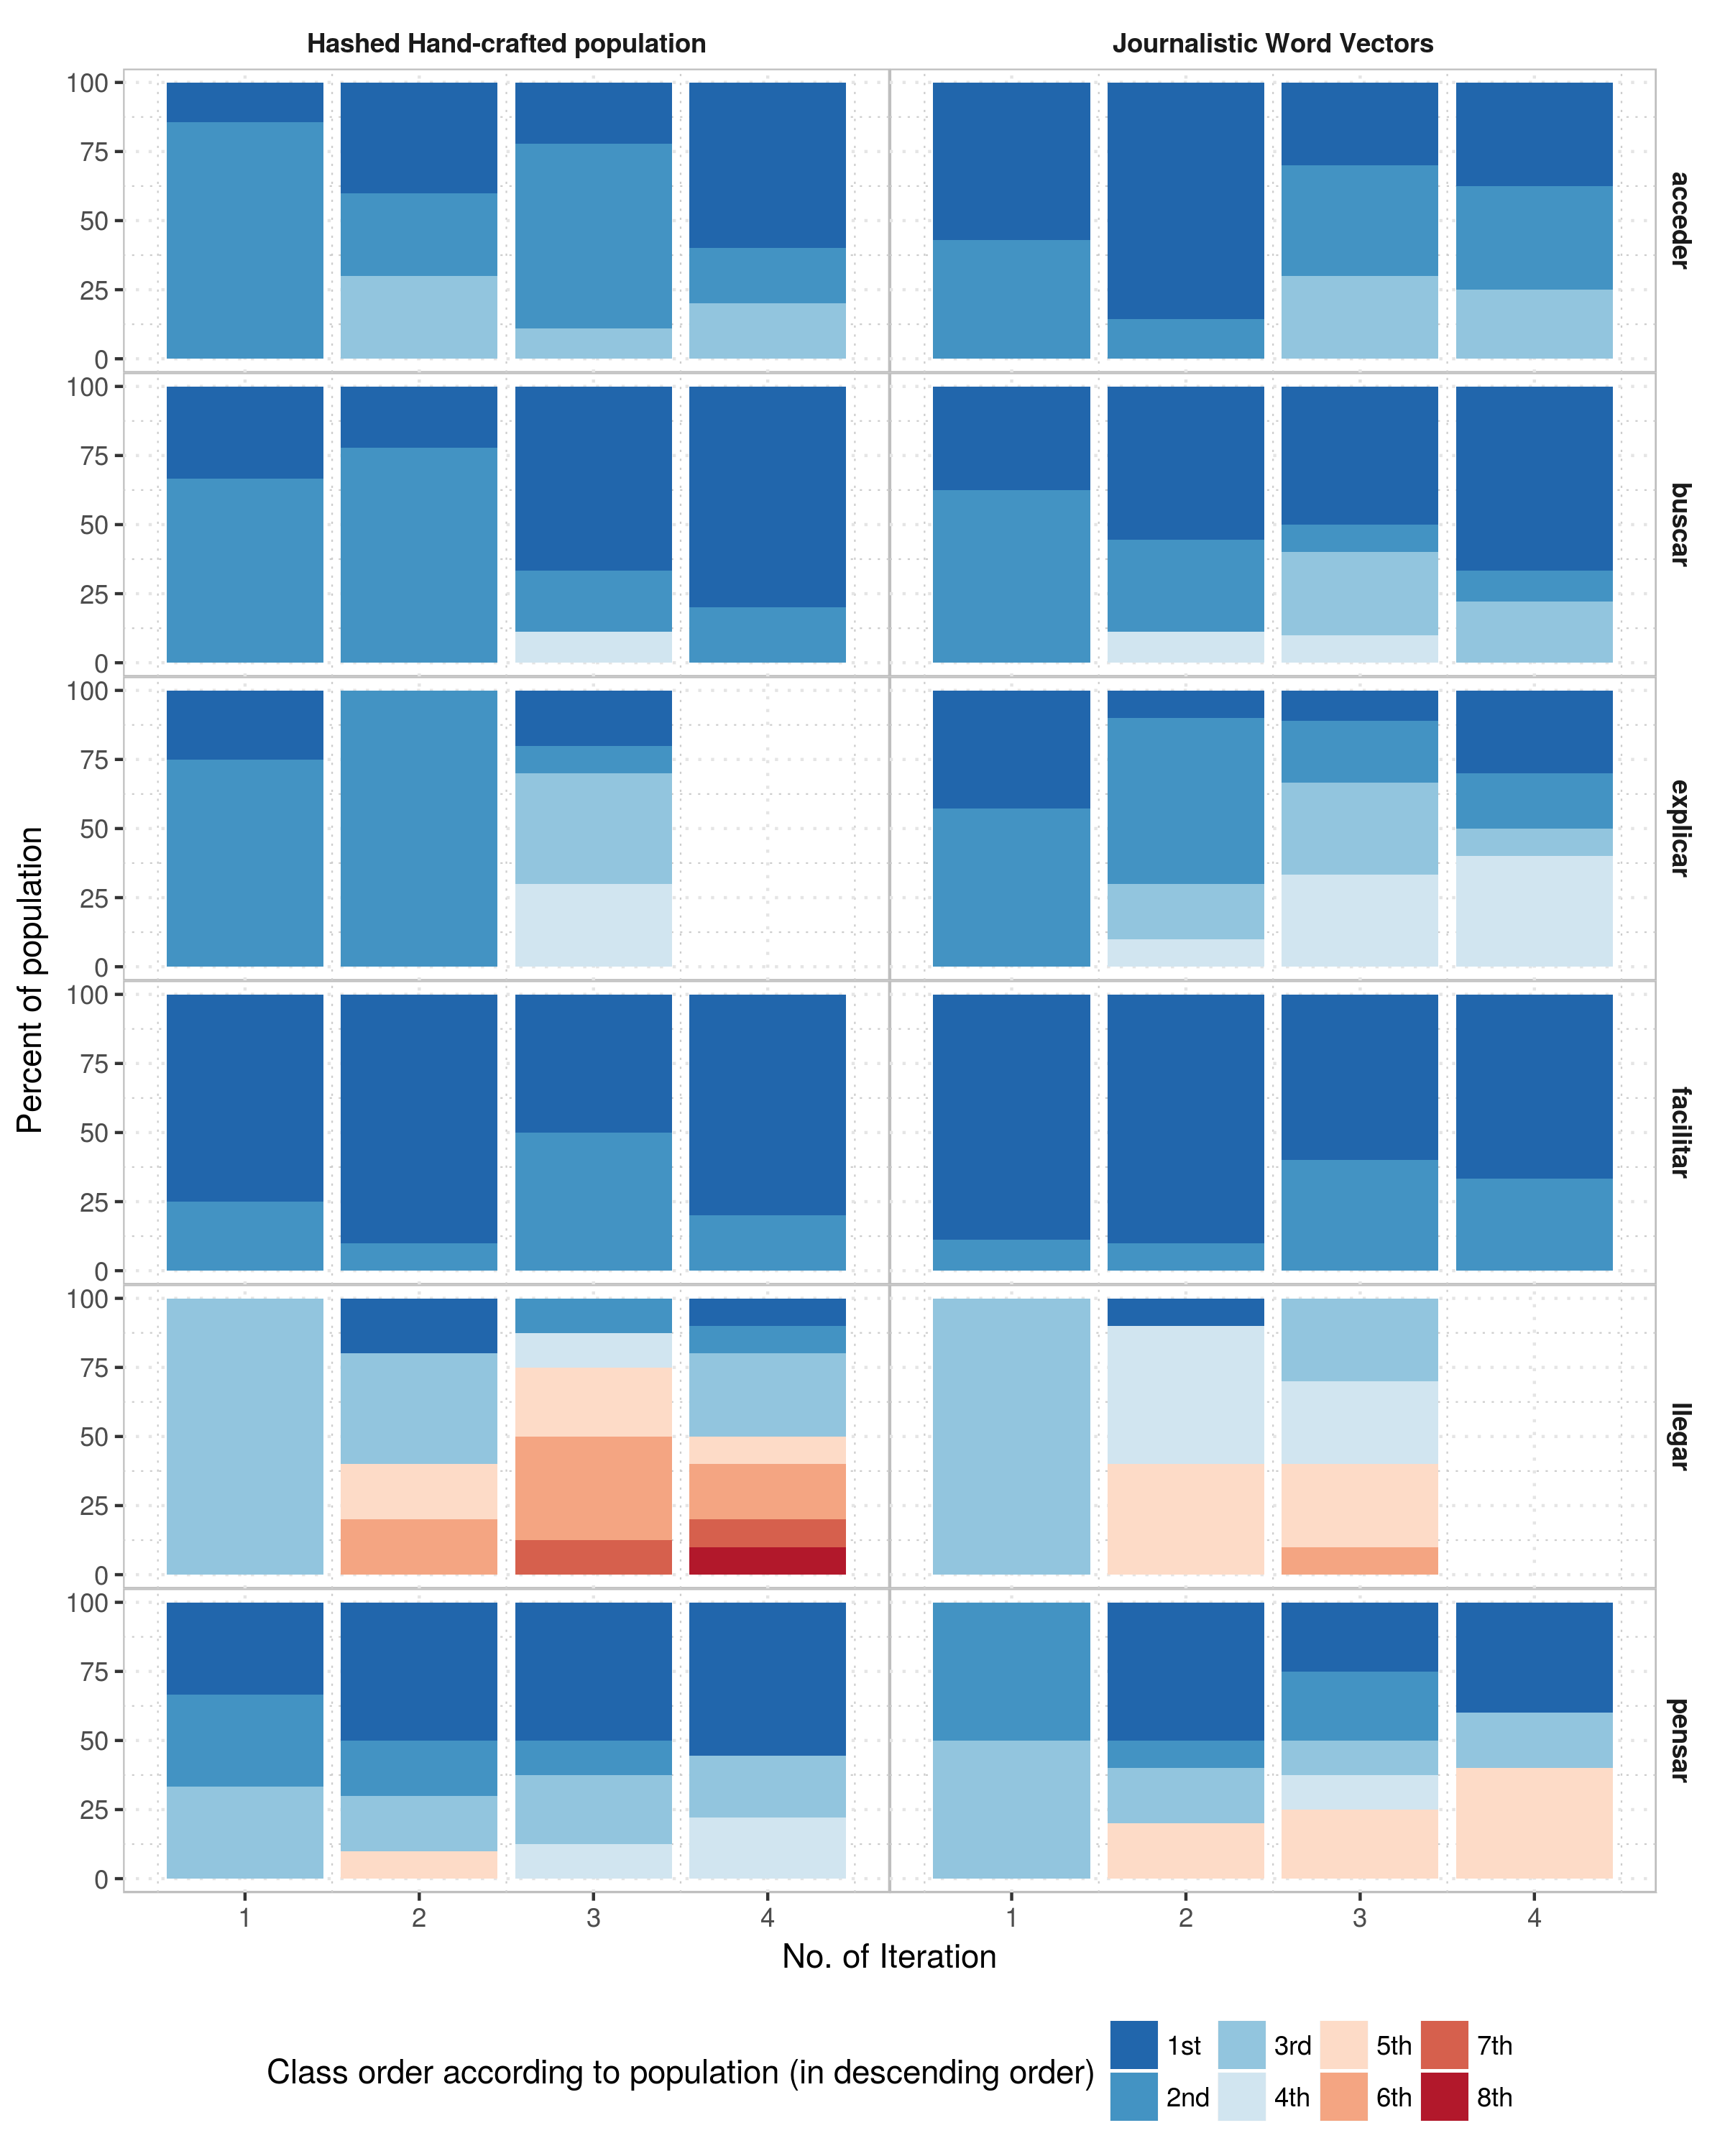
\includegraphics[height=0.9\textheight,width=\textwidth,keepaspectratio]
    {plots/active/population_add_per_class}
  \caption{Population added per sense on each iteration of active learning as a
  proportional count of all the examples added in that iteration}
  \label{fig:active:population_add_per_class}
\end{figure}

Figure \ref{fig:active:population_add_per_class} shows the proportion of
examples added per class on each iteration. It is a stacked bar plot where each
bar represents the total examples added in the iteration split by the
proportion of classes automatically annotated as such. The structure of the
plot is the following:

\begin{itemize}
  \item Each row shows the results for a token lemma: ``acceder'', ``buscar'',
    ``explicar'', ``facilitar'', ``llegar'', and ``pensar''.
  \item Each column stands for a feature representation: hand-crafted hashed
    features and journalistic word vectors.
  \item The x-coordinate represents the iteration in the self-learning
    algorithm.
  \item The y-coordinate represents the percentage of examples automatically
    annotated and added to the model.
  \item Each bar plot represents the distribution of the examples added in
    the iteration. Each color of the stacked bar represents the class
    which the examples were annotated.
\end{itemize}

In the figure there is a better view of what is happening along each iteration.
In general, the less frequent classes add more examples than the most frequent
class through iterations. This is a consequence of using uncertainty sampling,
which selects those classes near the decision border of the classifier.

In general, word embeddings are more uniform when adding examples of many
different classes. The consequence of this, I can hypothesize, is that for
hand-crafted features, and as a consequence of the low generalization they
have, the classifier is more certain about the most frequent class and thus
when applying the uncertainty sampling technique it choses mostly examples of
the less frequent classes. Word embeddings, on the other hand, have better
generalization from the start, thus when sampling elements with uncertainty it
can have low certainty also for some of the examples of the most frequent
class.

In any case, from these results I have enough evidence to support Hypothesis
\ref{hyp:active:1} which states that the distribution of the different classes
through the active learning algorithm iterations is maintained.

\subsection{Hypothesis \ref{hyp:active:2}}\label{sec:active:hyp:2}

I follow up with the test of Hypothesis \ref{hyp:active:2}. Recall that the
hypothesis states the active learning algorithm adds more information with the
examples it adds to the model in comparison to self-learning. This is a
consequence of the examples added being of classes the model has already less
information about due to the uncertainty sampling technique.

To test the Hypothesis I measure the results of Experiment \ref{exp:active:3},
which records the number of times a feature appears with a class. However, what
I am mostly interested about in this occasion is the total number of features
added per iteration of both self-learning and active learning algorithms. These
results are measured by Metric \ref{met:6} which is the normalized count of
features added in an iteration by the examples added in the same iteration.
The reason to use this measure instead of the raw count is because it is clear
that the number of features for self-learning will be higher than for active
learning since the number of examples that self-learning annotates in each
iteration is of a magnitude greater than active learning. However, what the
Hypothesis states, and what I am interested about, is whether these fewer
examples of the active learning algorithm actually add more information than
the self-learning algorithm.

\begin{figure}[htb!]
  \centering
  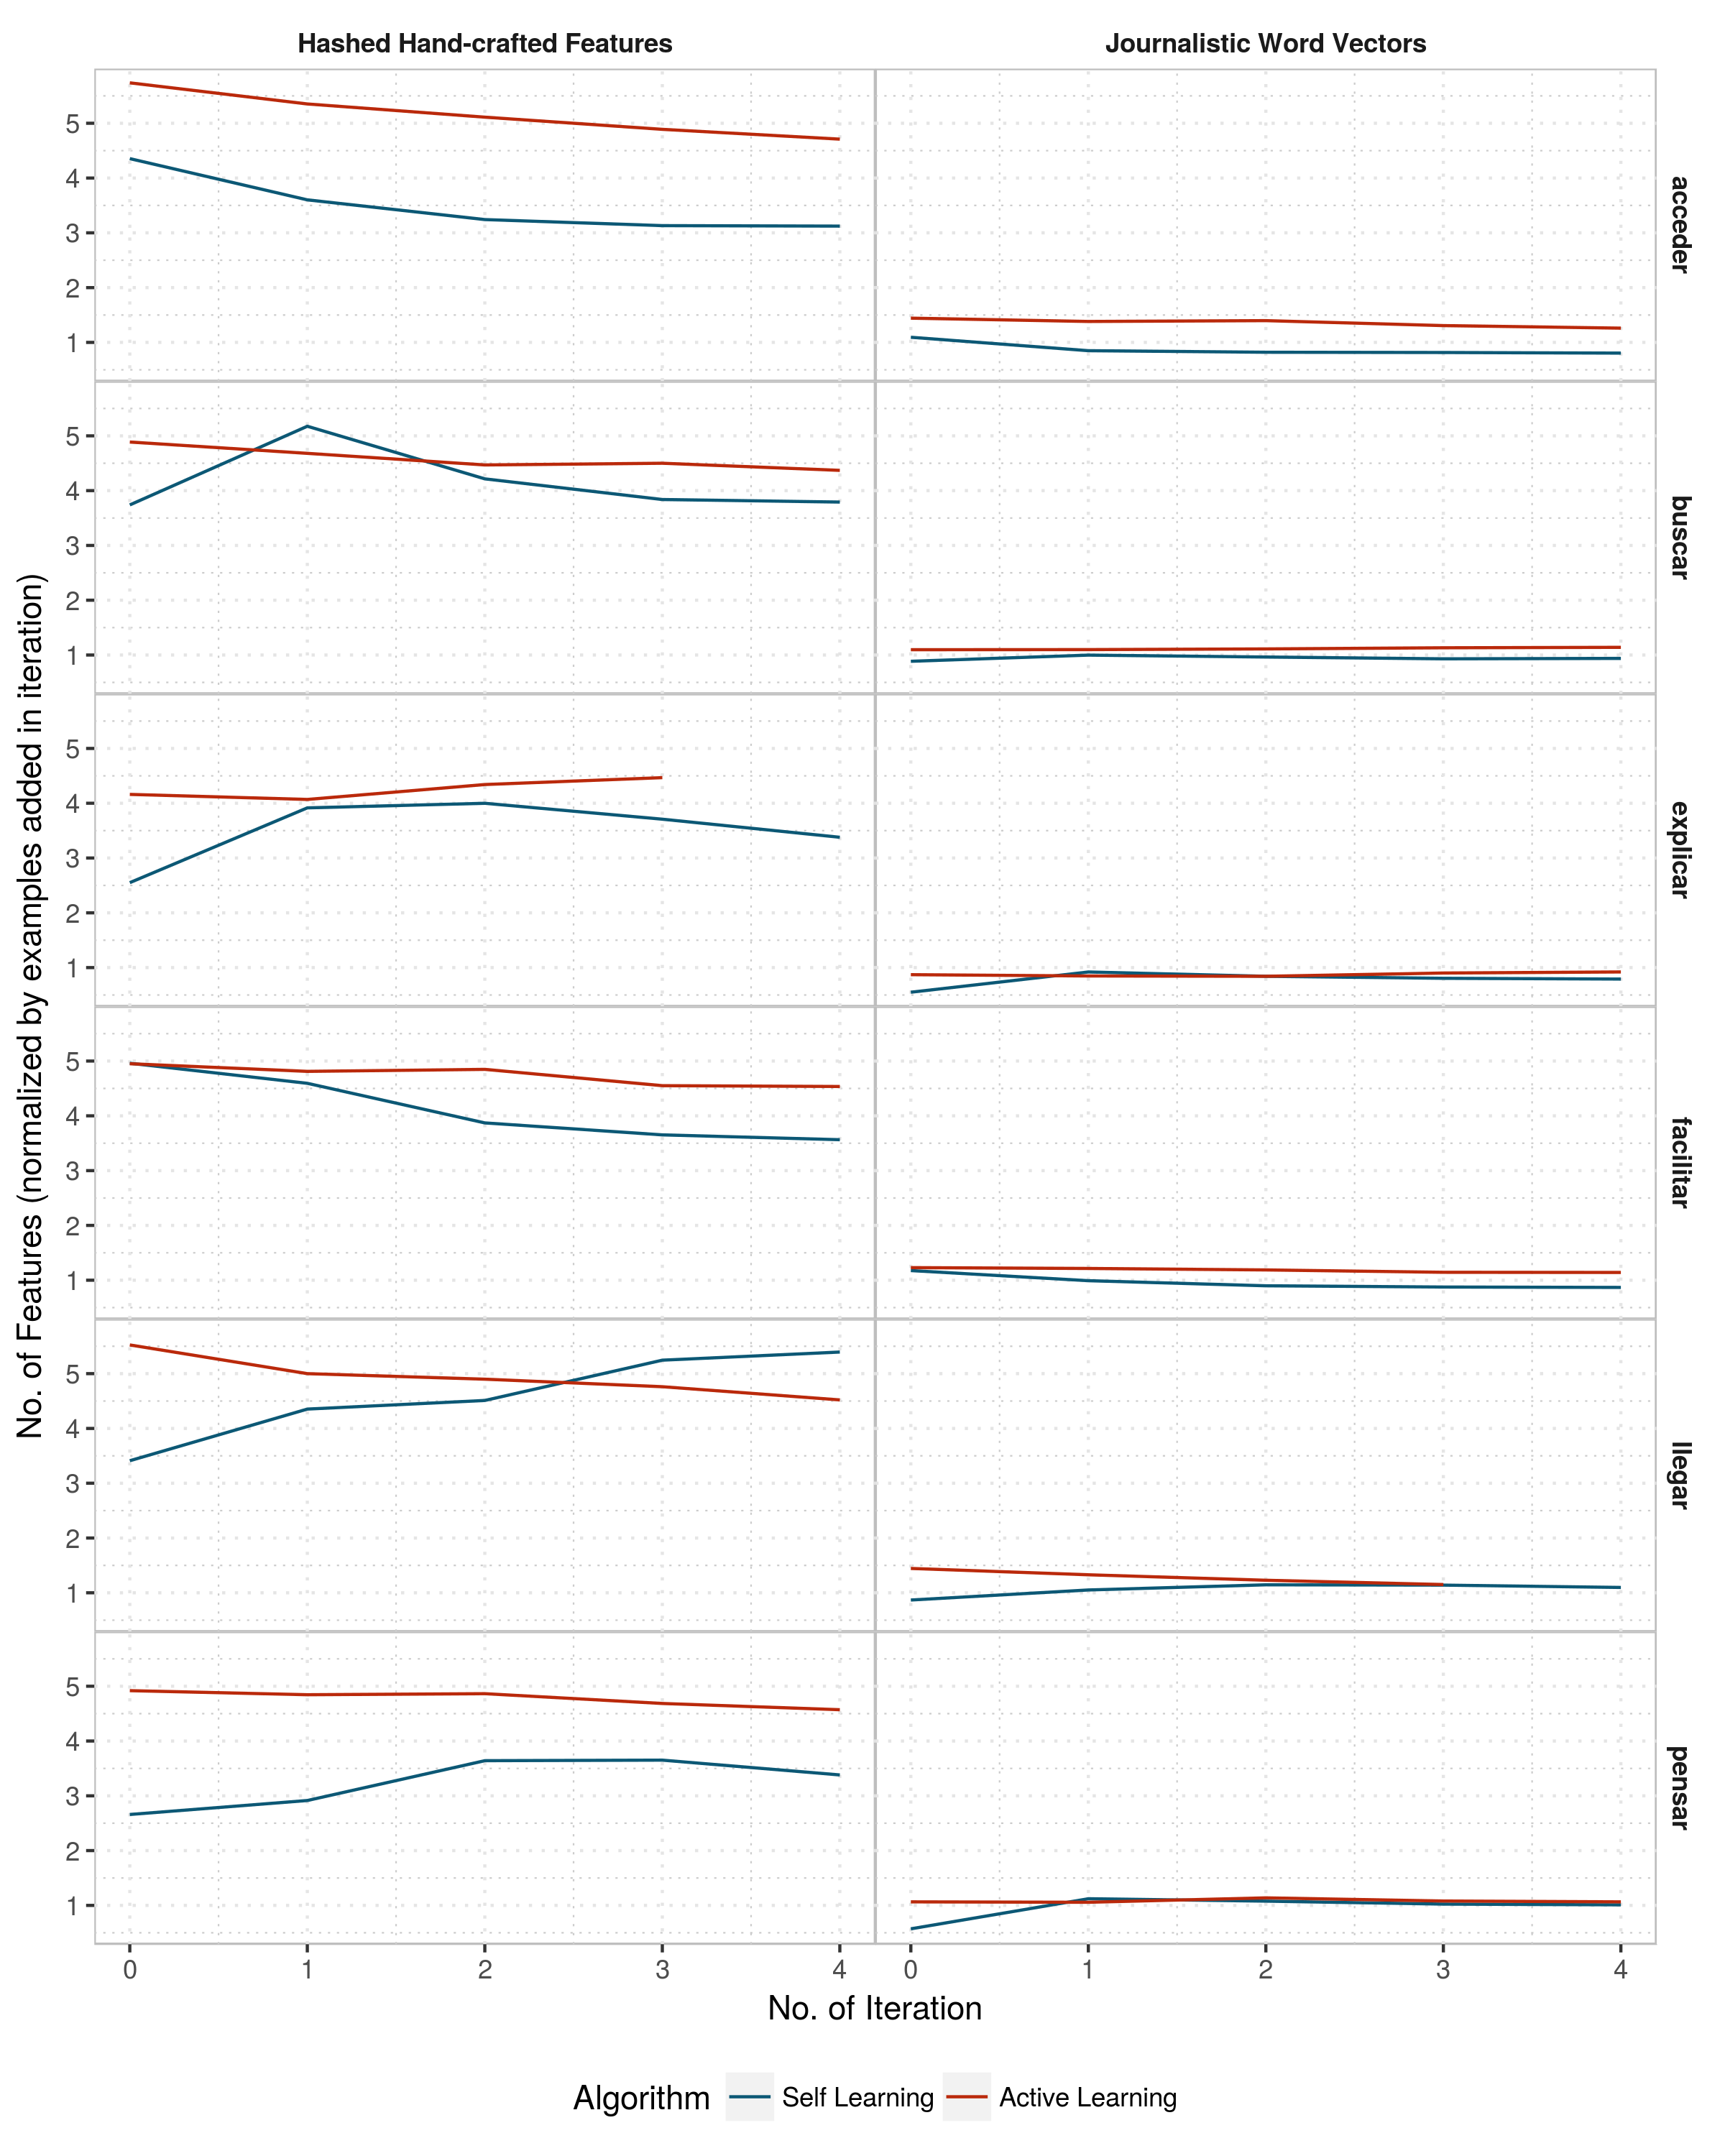
\includegraphics[height=0.9\textheight,width=\textwidth,keepaspectratio]
    {plots/active/feature_growth_comparison}
  \caption{Number of features added in each iteration of both self-learning
  and active learning. The features are normalized by the number of examples
  added in the iteration}
  \label{fig:active:feature_growth_comparison}
\end{figure}

Figure \ref{fig:active:feature_growth_comparison} shows the amount of features
added in each iteration of both self-learning and active learning normalized by
the amount of examples added. The structure of the graphic is as follows:

\begin{itemize}
  \item Each row shows the results for a token lemma: ``acceder'', ``buscar'',
    ``explicar'', ``facilitar'', ``llegar'', and ``pensar''.
  \item Each column stands for a feature representation: hand-crafted hashed
    features and journalistic word vectors.
  \item The x-coordinate axis represents the iteration number in the
    self-learning algorithm.
  \item The y-coordinate axis represents the normalized count of unique
    features by the number of examples added.
  \item Each line represents the number of features and the different colors
    represents the algorithm: self-learning and active learning.
\end{itemize}

The tendency shown in Figure \ref{fig:active:feature_growth_comparison} is
clear enough. Active learning is adding more information to the model by adding
more features per examples in comparison to self-learning. This is clearly a
consequence of active learning adding examples of less frequent classes in
contrast to self-learning as I showed in the previous Hypothesis's results.
Moreover, active learning is adding examples of classes that are non-existent
for self-learning since the classes are not part of the initial seed model.

For active learning, the most frequent class, which contains most of the
features in the initial model, is not the only one to grow in each iteration
(in fact, sometimes it is the one with the lowest number of examples added in
an iteration). Thus that class is not overtaking all the features added per
iteration. Then, when instances of classes with less occurrences are added the
data enriches more the model initial model. This can also be seen by inspecting
the PMI of the features and the classes, as in the next section.

\subsubsection{Features PMI}

There is another view for the results of Experiment \ref{exp:active:3}, that is
the one measured by the PMI defined in Metric \ref{met:5}, which associates the
features to the classes with a higher PMI and then gets the mean PMI per class.
In this section I show the results as measured by that metric and draw
conclusions regarding the Hypothesis.

\begin{figure}[htb!]
  \centering
  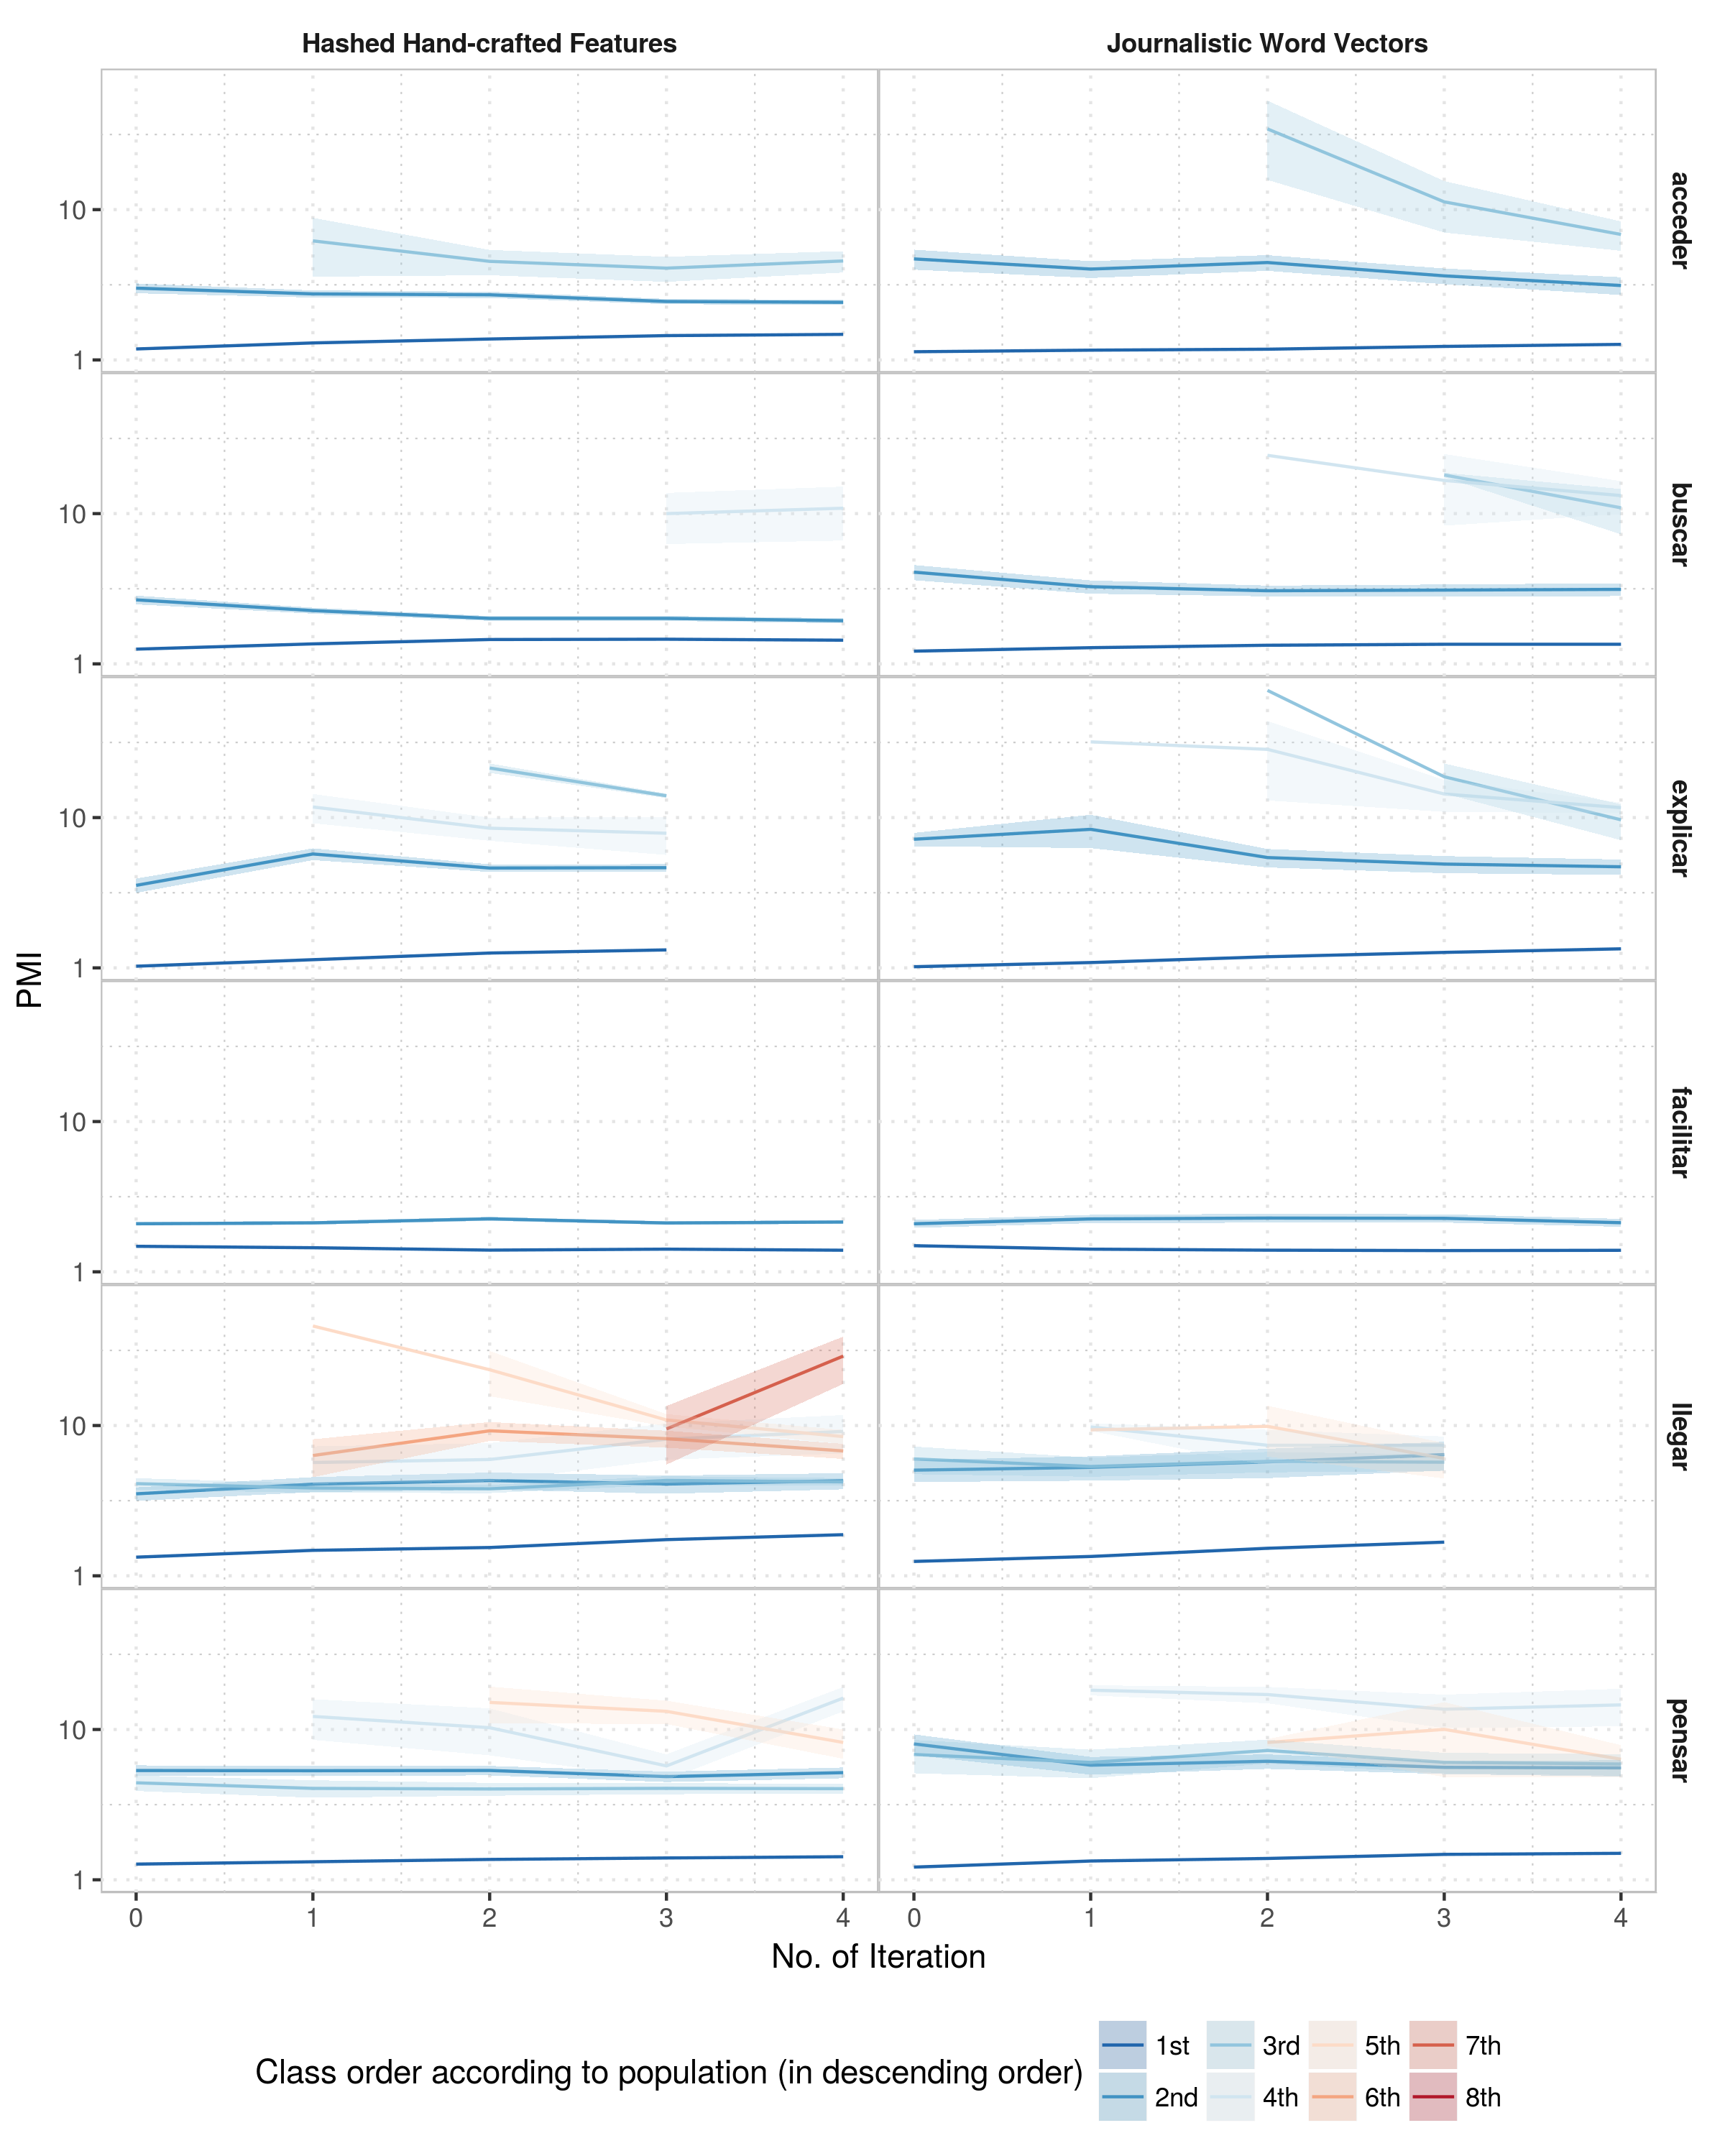
\includegraphics[height=0.9\textheight,width=\textwidth,keepaspectratio]
    {plots/active/features_pmi}
  \caption{Features pointwise mutual information with each of the classes
  across active learning iterations}
  \label{fig:active:pmi}
\end{figure}

Figure \ref{fig:active:pmi} displays the mean and standard error of the mean of
the pointwise mutual information between features and classes across the active
learning iterations. Recall that the metric associates features to the class it
has a larger PMI with. The figure shows a line plot with the following
structure:

\begin{itemize}
  \item Each row shows the results for a token lemma: ``acceder'', ``buscar'',
    ``explicar'', ``facilitar'', ``llegar'', and ``pensar''.
  \item Each column stands for a feature representation: hand-crafted hashed
    features and journalistic word vectors.
  \item The x-coordinate axis represents the iteration number in the
    self-learning algorithm.
  \item The y-coordinate axis represents the raw count of unique features in a
    logarithmic scale.
  \item Each color represents a class.
  \item The line of darker color in the middle represents the mean of the PMI
    for the class and the shadowed area represents the standard error of the
    mean for that PMI.
\end{itemize}

The figure shows that the mean of the PMI of the most frequent class with
respect to the features it is associated to is still the lowest one in
comparison to the rest of the classes. This is analogous to what happened in
self-learning and I already showed in Section
\ref{sec:self-learning:featurespmi}.

However, in contrast to what happened in self-learning, the PMI is not
decreasing in particular for the most frequent class or for those classes which
are consolidated in the model. It decreases for those new classes added through
the iterations which have few examples. This however may be a direct
consequence of Metric \ref{met:5} inadequately modeling classes with few
examples. In any case, the examples of classes unknown to the seed supervised
model have little information to start with, specially in the first iterations
after they first occur. In some cases, where there is no shadowed area is
because the examples added for such class are less than 3 total, thus it
does not have any variance.

The fact that the PMI of the consolidated classes (those appearing in the
original supervised dataset) does not decrease contrasts with what I showed for
self-learning. Since active learning does not drift to add only examples of
the most frequent class, then we have that the class does not drag noise by
adding features that are not necessarily from the class. That is, whichever
information is present in the class is maintained as the number of examples
increases.

I can conclude that the way new examples are incorporated to the model is
radically different for each algorithm. Self-learning adds as examples of the
most frequent class those instances weakly defined for the mere weight that
class has in the model decisions. This weakly defined instances blur the
decision boundaries the model has over that class. In contrast, the strategy
based on uncertainty sampling is oriented precisely to increase the definition
of the decision boundary.

From the results seen in this Section it is safe to assume Hypothesis
\ref{hyp:active:2} has enough evidence to be accepted.

\section{Conclusions}\label{sec:active:conclusions}

The experiments I did in this chapter had very little data because of the extra
cost of annotating examples, necessary for active learning. I decided to go
further with this option instead of doing some sort of simulation based on the
already annotated examples since the labeled dataset was so small that
selecting examples in that universe invalidates one of the assumptions of
active learning, which is obtaining the examples from the universe which will
maximize the learning in the model. This is because the number of possible
examples using a simulation like that does not cover enough of the universe of
possible examples.

First of all, active learning shows better general performance than
self-learning, by showing better results in the held-out test corpus. This is
not only for the most frequent class but for some of the less frequent classes
as well. This better performance can be explained by the results obtained to
accept both hypotheses of the chapter.

Experimental results lead me to accept Hypothesis \ref{hyp:active:1}. The model
for active learning maintains the representativity in the data through the
algorithm, unlike what happened with self-learning, where the new examples were
added as part of the most frequent class. In particular, the less frequent
classes are the ones to benefit the most with this model as a consequence of
the nature of the uncertainty sampling technique itself, which selects for
annotation the instances the model has less information about.

Hypothesis \ref{hyp:active:2} can also be accepted according to experimental
results. The tendency shows that active learning adds in each iteration more
information than self-learning, taking into account the number of examples it
adds in each iteration. Indeed, the model adds more information by adding more
new features per example, which also happen to be more informative of the
classes, specially the less frequent ones (this is what is shown when PMI is
graphically displayed). This way there are clearer boundaries for the less
frequent classes and, reciprocally, in the most frequent class as well. In
contrast, I had found that self-learning associates new features mostly to the
most frequent class and thus weakening the decision boundaries the model had
over it.

Again this are only preliminary results and the conclusions I could draw from
them are only tentative. To do a more thorough study I should annotate more
data with the aid of a domain expert and see how these results are expanded
with more iterations. A possible hypothesis to develop in this sense is that
eventually the less frequent classes will find an upper bound for the model to
have enough certainty over each of the less frequent classes. In that moment,
the algorithm will start to converge and will select instances from the
unlabeled pool of almost all classes uniformly.

In any case the main conclusion from this chapter is that active learning is an
interesting source to extend the coverage of a model. It does not suffer from
the fundamental problem of self-learning, namely the drift to the most frequent
class. This is a direct consequence of the way the instances to annotate are
selected by the algorithm. Indeed, this selection of instances plus the added
value of a domain expert doing the annotation instead of the algorithm itself
based on certainty, results in a more robust model with more information on
classes it originally had little to no information about.

However, there are still challenges left. First, the annotation process is
costly. In comparison to self-learning, which does the annotation
automatically, active learning requires a human doing manual labor. Although
the algorithm tries to select those instances having the highest impact in the
model, the manual labor is still expensive. Moreover, the annotation is not
easy, as I explained in Section \ref{sec:active:difficulties}, because the
resource is not perfect as it is arbitrary in some aspects like the granularity
of the senses or what senses are considered.

In the next chapter of this thesis I will explore yet another joint learning
technique. In that case the algorithm is not a wrapper over some supervised
classifier which adds unannotated data to the model. The algorithm named {\em
ladder networks} is an algorithm that minimizes two different objectives, one
for the supervised data and another for the unsupervised data. The algorithm
does the whole process automatically, in contrast to active learning, but as it
does not add the noise of examples as labeled dataset it does not drift to the
most frequent class as self-learning does.

The future work of this chapter will focus on doing more thorough
experimentations, using more annotation resources. In particular I want to
focus on two main aspects: how much does the number of annotations per
iteration affects the final outcome, and how much annotation is needed to be
done in order to have better representation for each class. More future work
is checking on other techniques for selecting the examples of active learning.
In particular, a comparison between selecting the instances with less certainty
and selecting random instances.

I also did some preliminary work on combining both active learning with
self-learning to attack the problem of the most frequent class drifting by
constantly adding examples manually via uncertainty sampling and an oracle.
However this work was not further explored in this thesis and is left out as
future work as well.

